% =====================================================================
% RMSTSS A0 Landscape Poster (Improved Layout & Color Sections)
% =====================================================================
\documentclass[a0,landscape]{a0poster}

% ---------------------------------------------------------------------
% PACKAGES
% ---------------------------------------------------------------------
\usepackage{helvet}                % Helvetica (sans-serif)
\usepackage[dvipsnames]{xcolor}    % Extended colors
\usepackage{graphicx}              % Include graphics
\usepackage{geometry}              % Page geometry
\usepackage{qrcode}                % QR codes
\usepackage{amssymb}               % Math symbols
\usepackage{alltt}                 % Verbatim-ish environment
\usepackage{tikz}                  % TikZ for backgrounds
\usetikzlibrary{shapes.geometric, arrows.meta}
\usepackage{setspace}              % Line spacing
\usepackage[compact]{titlesec}     % Heading spacing
\usepackage{enumitem}              % List control
\usepackage{pifont}                % \\ding symbols

% --- Custom Colors ---
\definecolor{HeadingColor}{RGB}{0, 90, 110}   % Teal for headings
\definecolor{BulletColor}{RGB}{220,50,47}     % Red for cross marks

\newcommand{\xmark}{\ding{55}}              % Cross symbol

\renewcommand{\familydefault}{\sfdefault}

\geometry{papersize={35in,45in}, margin=1in, top=1in, bottom=1in}

\setstretch{0.95}
\setlist{nosep}
\titlespacing*{\subsection}{0pt}{1ex}{0.5ex}

\begin{document}

\begin{tikzpicture}[remember picture, overlay]
    % Header background changed to an orange gradient
    \shade[top color=Orange!0, bottom color=Orange] 
        (current page.north west) rectangle ([yshift=-3.25in]current page.north east);
    
    % Other background sections remain unchanged
    \fill[gray!20] (current page.south west) rectangle ([yshift=4in]current page.south west |- current page.south east);
    \shade[top color=cyan!5, bottom color=teal!50]
        ([yshift=-6in]current page.north west) rectangle ([yshift=4in]current page.south east);
\end{tikzpicture}

\noindent
% Start of the first minipage for the logo (left column)
\begin{minipage}[c]{0.2\linewidth}
    \centering
    
\includegraphics[height=5cm, width=\linewidth,height = \linewidth]{images/UTHSC-logo.png}
\end{minipage}
\begin{minipage}[c]{0.6\linewidth}
    \centering 
    \fontsize{60}{66}\selectfont \textbf{\color{HeadingColor}A Software Tool for Planning Better Clinical Trials} \\
    \huge \textbf{Arnab Aich, Yuan Zhang} \\
    \huge \textit{Department of Preventive Medicine}
\end{minipage}%
\begin{minipage}[c]{0.2\linewidth}
    \centering
    
\includegraphics[height= 0.8\linewidth, width=0.8\linewidth]{images/app-qr-code.png}
\end{minipage}
 \hfill
\vspace{0.2cm}
%\rule{\linewidth}{1.5pt}

\begin{minipage}[t]{0.44\linewidth}

    \subsection*{\color{HeadingColor}\huge Key Questions in Clinical Trials}
    {\centering 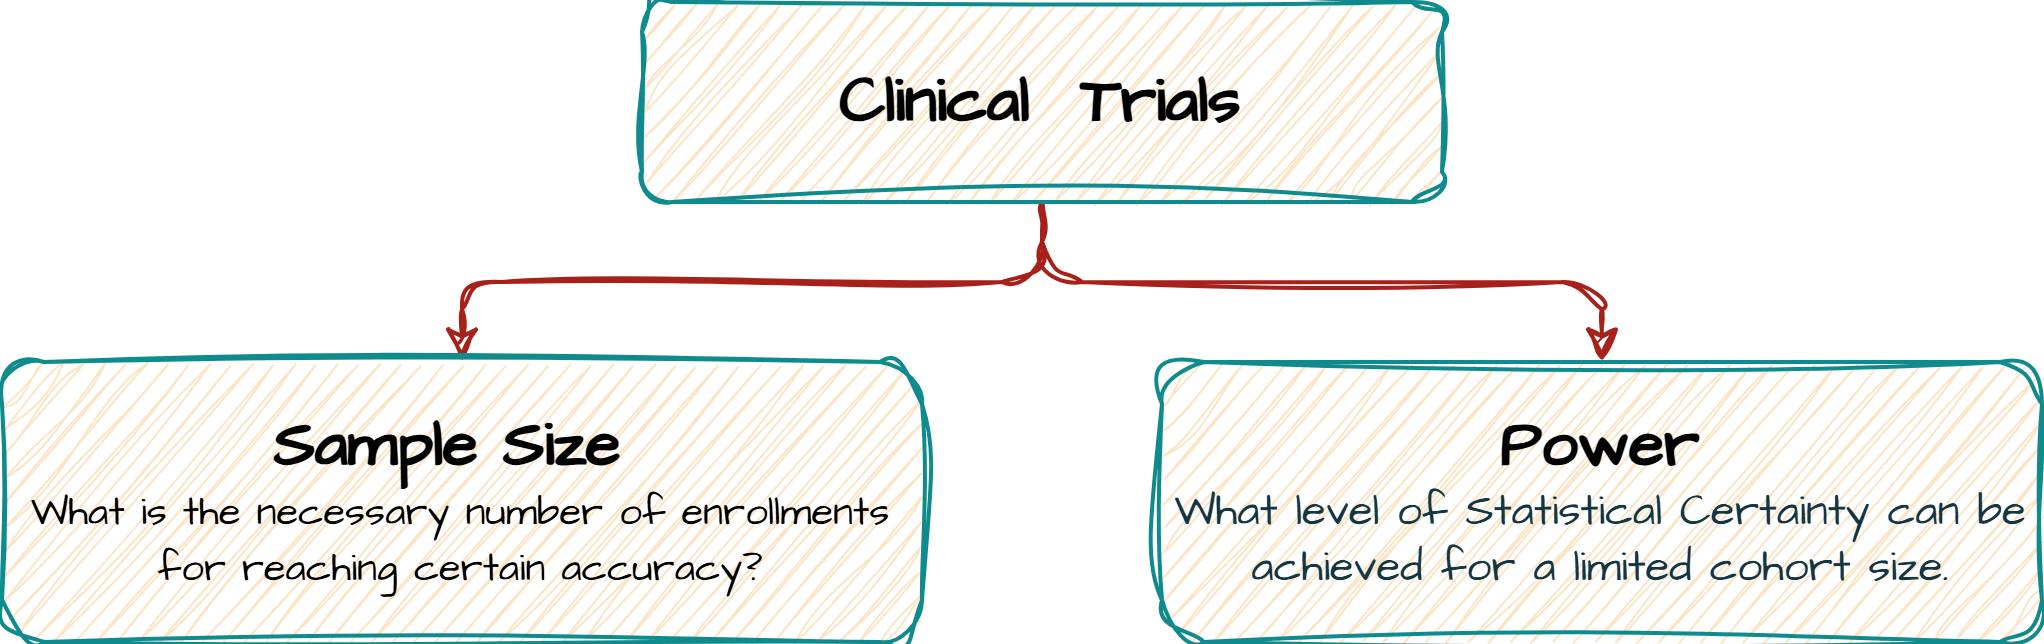
\includegraphics[width=\linewidth,height = 0.5\linewidth]{images/CT-intro.png}\par}

    \subsection*{\color{HeadingColor}\huge Problems in Traditional Methods}
    \Large In general, Survival clinical trials (\textit{Time to event}) relies on the \textbf{HR} (Hazard Ratio).
   \begin{itemize}[label={\color{BulletColor}\Large \xmark}]
    \item \Large Depends on strong assumptions, violated in the real world.
    \item \Large Identifying treatment benefits are challenging.
\end{itemize}
\hfill
    \subsection*{\color{HeadingColor}\huge Solution: Restricted Mean Survival Time}
    \begin{itemize}
        \item[{\color{BulletColor}\Large\checkmark}] \Large Directly measures the average \textbf{event-free} time of patients.
        \item[{\color{BulletColor}\Large\checkmark}] \Large Do not use additional assumptions.
        \item[{\color{BulletColor}\Large\checkmark}] \Large It is easy for everyone to understand.
        \item[{\color{BulletColor}\Large\checkmark}] \Large It provides a clear measure of treatment benefit.
    \end{itemize}
    \hfill
  \vspace{0.2cm}    
    {\centering 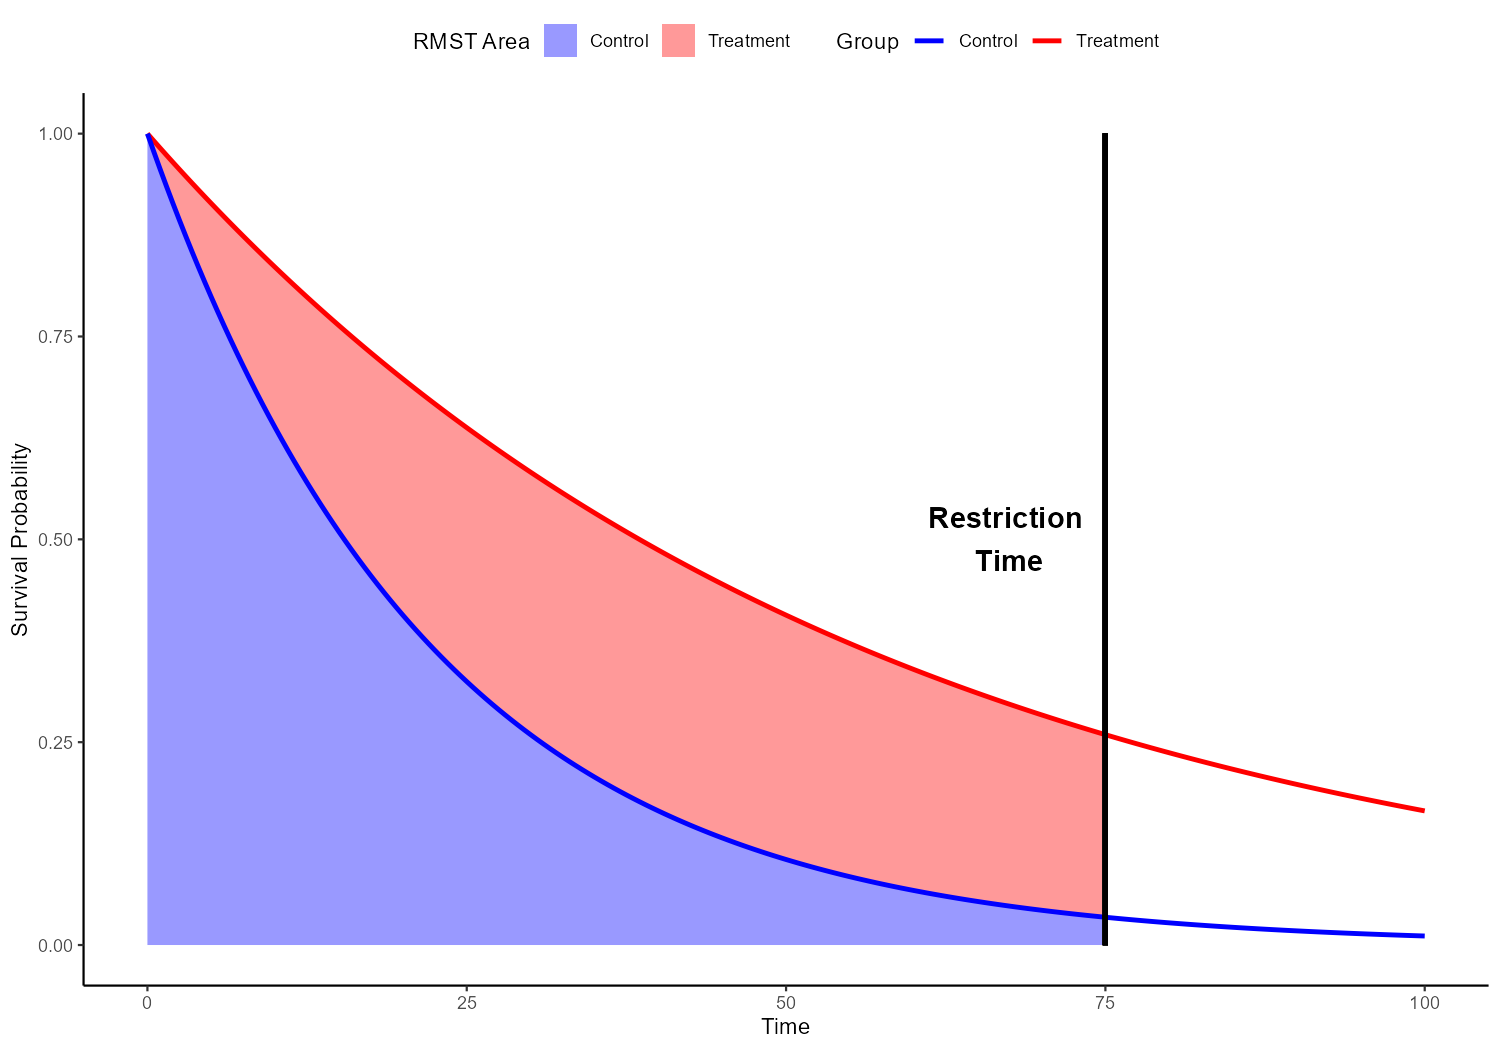
\includegraphics[width=\linewidth,height = 0.75\linewidth]{images/rmst_causal_plot.png}\par}
\end{minipage}
\hfill
\begin{minipage}[t]{0.54\linewidth}
    \subsection*{\color{HeadingColor}\huge What We Are Offering}
    {\centering 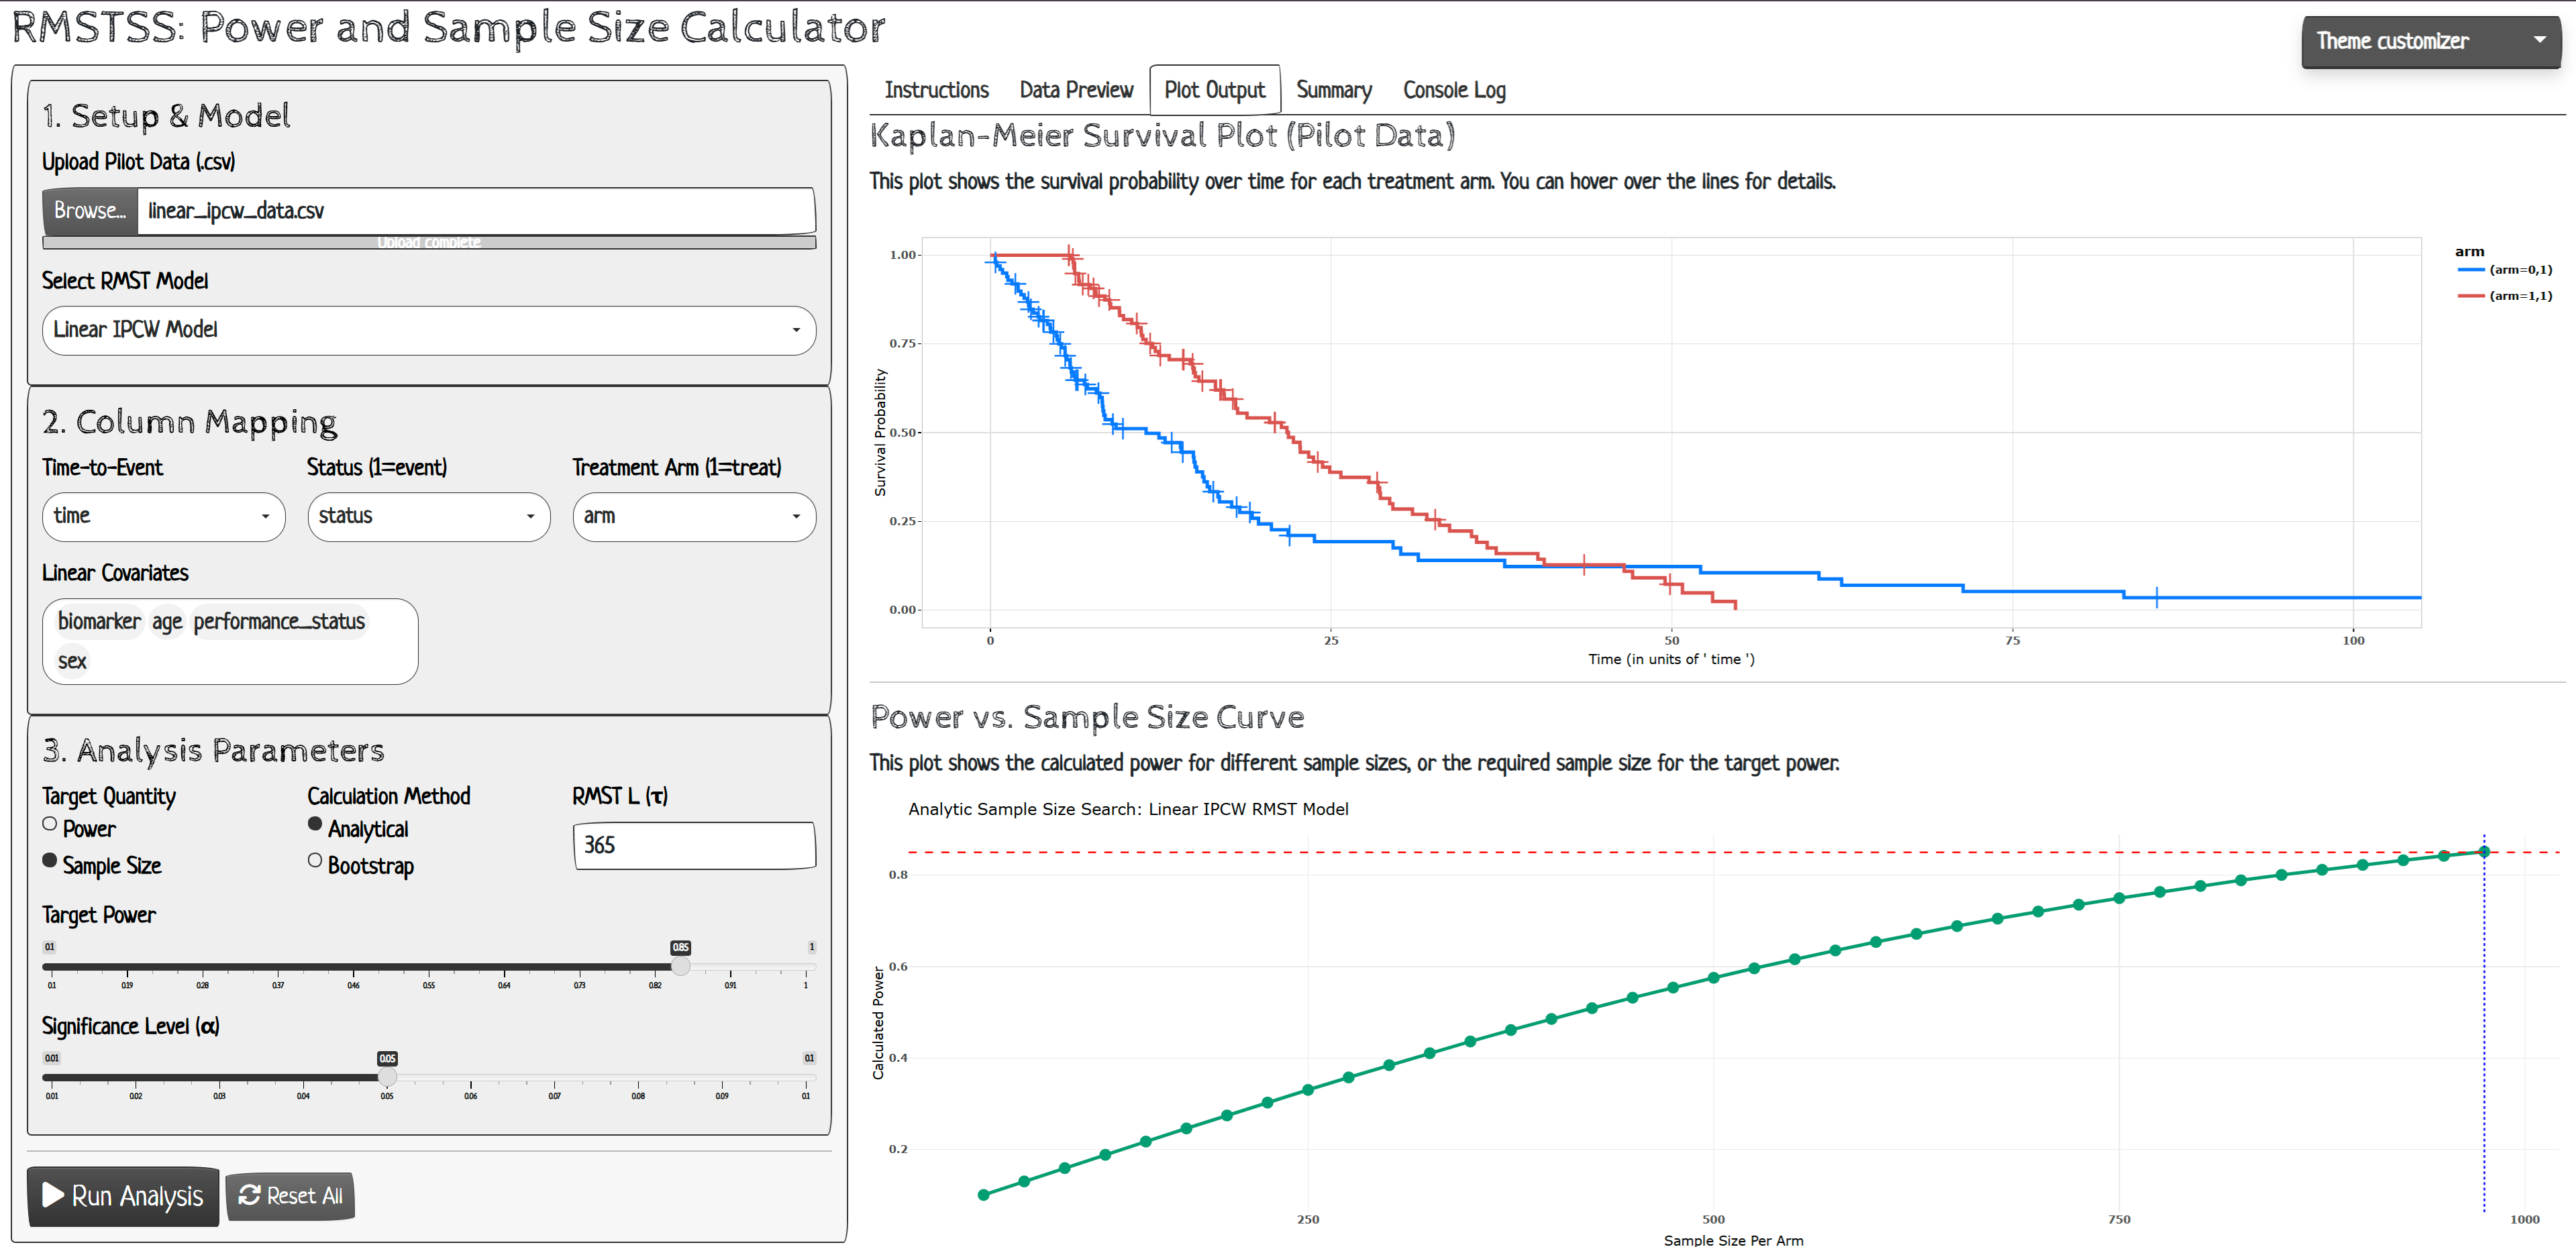
\includegraphics[width=\linewidth,height = 0.65\linewidth]{images/app-ss.png}\par}

\vspace{2cm}    
    \subsection*{\color{HeadingColor}\huge App Features}
    \begin{itemize}
        \item[{\color{BulletColor}\Large\checkmark}] \Large \textbf{Variable Selection:} Choose covariates to add in model.
        \item[{\color{BulletColor}\Large\checkmark}] \Large \textbf{Flexible Methods:} Use a \textbf{Quick Check} (Analytical) or a \textbf{Deep Dive}(Bootstrap).
        \item[{\color{BulletColor}\Large\checkmark}] \Large \textbf{Downloadable Reports:} Generate an HTML report.
        \item[{\color{BulletColor}\Large\checkmark}] \Large \textbf{Customization:} Change themes, fonts, size, and many more on the go.
    \end{itemize}
\vspace{2cm}    
\hfill
    {\centering 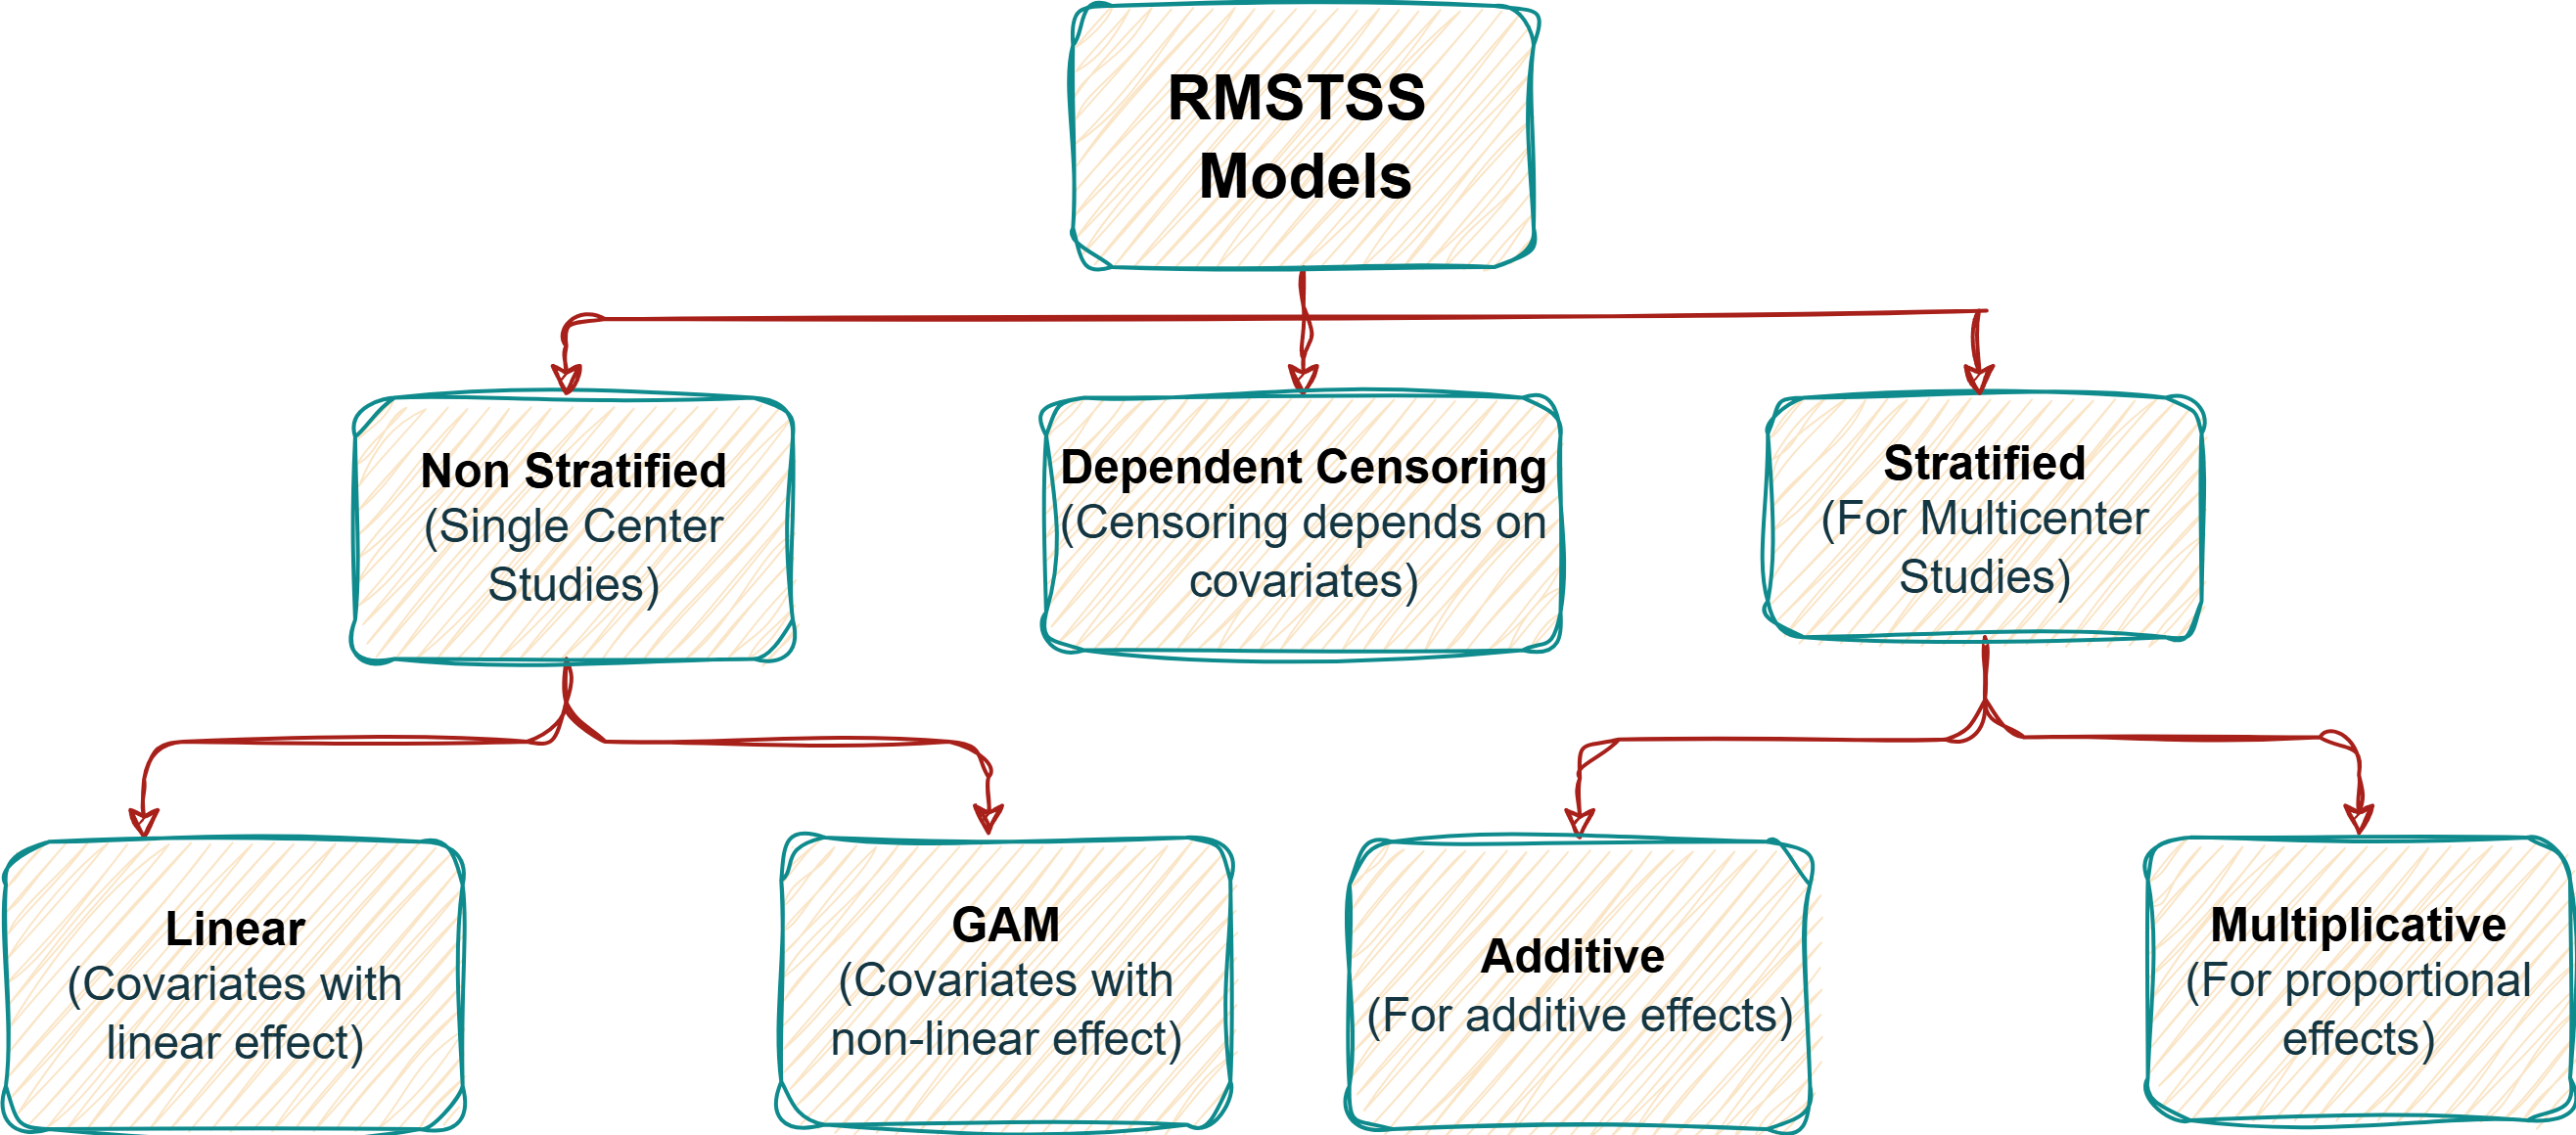
\includegraphics[width=\linewidth,height = 0.6\linewidth]{images/app-models.png}\par}
\end{minipage}

\hfill
\rule{\linewidth}{2.5pt} % Horizontal line to separate footer

\begin{minipage}[t]{0.5\linewidth}
    \subsection*{\Large For Statisticians and Programmers}
    \Large We also developed an \textbf{R-Package} for function-level interaction. After installing the package from GitHub, the app can be run locally using the \verb|RMSTSS::run_app()| function call. For package website scan the QR code.
\end{minipage}
\hfill
\begin{minipage}[c]{0.1\linewidth}
    \centering
    
\includegraphics[height=\linewidth, width=\linewidth]{images/package-qr-code.png}
\end{minipage}
\hfill
\begin{minipage}[t]{0.3\linewidth}
    \subsection*{\Large Acknowledgments}
    \begin{enumerate}
        \item \Large NSF grant no. 2220726.
        \item \Large UTHSC BERD (Biostatistics, Epidemiology and Research Design).
    \end{enumerate}
\end{minipage}
\end{document}
